\documentclass[review,12pt]{elsarticle}
\usepackage[T1]{fontenc}
\usepackage[utf8]{inputenc}
\usepackage{amsmath,amssymb,amsthm,booktabs,graphicx,microtype}
\usepackage{xurl}
\usepackage[hidelinks]{hyperref}
\newtheorem{proposition}{Proposition}
\newtheorem{corollary}{Corollary}
\newcommand{\ind}{\mathbf{1}}
\newcommand{\StaticNoneHit}{49.7}
\newcommand{\StaticNoneRetention}{100.0}
\newcommand{\StaticNoneCoverage}{98.5}
\newcommand{\StaticNonePeak}{51.9}
\newcommand{\StaticBspHit}{7.4}
\newcommand{\StaticBspRetention}{48.7}
\newcommand{\StaticBspCoverage}{96.9}
\newcommand{\StaticBspPeak}{8.0}
\newcommand{\StaticAblationHit}{10.1}
\newcommand{\StaticAblationRetention}{51.6}
\newcommand{\StaticAblationCoverage}{96.9}
\newcommand{\StaticAblationPeak}{10.2}
\newcommand{\StaticRandomHit}{21.5}
\newcommand{\StaticRandomRetention}{49.1}
\newcommand{\StaticRandomCoverage}{98.1}
\newcommand{\StaticRandomPeak}{22.5}
\newcommand{\WalkNoneHit}{16.4}
\newcommand{\WalkNoneRetention}{100.0}
\newcommand{\WalkNoneCoverage}{95.3}
\newcommand{\WalkNonePeak}{16.1}
\newcommand{\WalkBspHit}{5.9}
\newcommand{\WalkBspRetention}{48.9}
\newcommand{\WalkBspCoverage}{94.9}
\newcommand{\WalkBspPeak}{6.8}
\newcommand{\WalkAblationHit}{6.5}
\newcommand{\WalkAblationRetention}{47.1}
\newcommand{\WalkAblationCoverage}{95.7}
\newcommand{\WalkAblationPeak}{7.3}
\newcommand{\WalkRandomHit}{7.9}
\newcommand{\WalkRandomRetention}{48.6}
\newcommand{\WalkRandomCoverage}{94.3}
\newcommand{\WalkRandomPeak}{7.9}
\newcommand{\CommuteNoneHit}{7.8}
\newcommand{\CommuteNoneRetention}{100.0}
\newcommand{\CommuteNoneCoverage}{78.4}
\newcommand{\CommuteNonePeak}{13.4}
\newcommand{\CommuteBspHit}{3.9}
\newcommand{\CommuteBspRetention}{54.4}
\newcommand{\CommuteBspCoverage}{82.5}
\newcommand{\CommuteBspPeak}{6.7}
\newcommand{\CommuteAblationHit}{4.2}
\newcommand{\CommuteAblationRetention}{54.1}
\newcommand{\CommuteAblationCoverage}{82.4}
\newcommand{\CommuteAblationPeak}{7.2}
\newcommand{\CommuteRandomHit}{4.8}
\newcommand{\CommuteRandomRetention}{50.6}
\newcommand{\CommuteRandomCoverage}{81.8}
\newcommand{\CommuteRandomPeak}{7.7}
\newcommand{\GeolifeNoneHit}{35.6}
\newcommand{\GeolifeNoneRetention}{100.0}
\newcommand{\GeolifeNoneCoverage}{94.0}
\newcommand{\GeolifeNonePeak}{35.8}
\newcommand{\GeolifeBspHit}{2.4}
\newcommand{\GeolifeBspRetention}{49.4}
\newcommand{\GeolifeBspCoverage}{92.7}
\newcommand{\GeolifeBspPeak}{7.9}
\newcommand{\GeolifeAblationHit}{1.8}
\newcommand{\GeolifeAblationRetention}{44.7}
\newcommand{\GeolifeAblationCoverage}{93.3}
\newcommand{\GeolifeAblationPeak}{9.3}
\newcommand{\GeolifeRandomHit}{16.5}
\newcommand{\GeolifeRandomRetention}{55.6}
\newcommand{\GeolifeRandomCoverage}{94.0}
\newcommand{\GeolifeRandomPeak}{14.8}

\newcommand{\PopulationPriorHit}{25.75}
\newcommand{\PopulationPriorPeak}{22.37}
\newcommand{\ReplayStaticWindows}{17}
\newcommand{\ReplayMedianCells}{3}
\newcommand{\LargeTaskShareMin}{83.7}
\newcommand{\LargeTaskShareMax}{90.5}
\newcommand{\RawCompletionMin}{4.69}
\newcommand{\RawCompletionMax}{5.33}

\journal{Pervasive and Mobile Computing}
% Use a plain first-page footer: this draft has not been submitted.
\makeatletter\let\ps@pprintTitle\ps@plain\makeatother
\begin{document}
\begin{frontmatter}
\title{Branch-Safe Participation under Model Uncertainty\\for Sequential Mobile Crowdsensing}
\author[aff1]{Lili He}
\author[aff1]{Sheng Jiang}
\author[aff1]{Linghui Lyu}
\author[aff1]{Lei Zhang\corref{cor1}}
\ead{8213662@163.com}
\cortext[cor1]{Corresponding author.}
\address[aff1]{College of Information and Electronic Technology, Jiamusi University, Jiamusi 154007, China}
\begin{abstract}
Keeping precise coordinates on a mobile device does not eliminate the location information carried by successful region-constrained sensing tasks, while silence can also update an observer's belief. We study this binary channel for linkable accounts under uncertain delivery, participation, and timely completion. A branch-safe participation (BSP) filter limits maximum posterior mass after either output; we derive its maximal scalar gate and a model-conditional sequential bound. We then extend BSP to a finite public ambiguity set: robust BSP (R-BSP) takes the minimum feasible gate across candidate Bayesian models and is the maximal common scalar gate satisfying every member's two-branch constraints. A software evaluation combines synthetic mobility and replay of 67 GeoLife users excluded from model fitting. At opportunity retention 0.5, exploratory test-selected envelopes give static-scenario MAP hit-rate reductions of 8.8 and 10.6 percentage points against task-channel adaptations of PML and PRIVIC; other scenarios show no consistent advantage over both. A post-hoc 20-seed stress test exposes the reason for the robust extension: at $\rho=0.1$, better-informed attacks produce local-cap violation rates up to 14.6\% for misspecified nominal BSP, whereas a nine-model R-BSP ensemble containing the attacker's model has zero observed local violations across five evaluated model conditions, with opportunity retention reduced to 39.7\%. Completed tasks remain dominated by large regions, and a development-fitted no-output predictor outperforms the uniform-prior replay inference reported under BSP. The resulting guarantee is finite-model and channel-specific, not protection against arbitrary auxiliary knowledge.
\end{abstract}
\begin{keyword}
Mobile crowdsensing \sep location privacy \sep Bayesian inference \sep adaptive tasks \sep participation filtering \sep reproducible simulation
\end{keyword}
\end{frontmatter}
\section{Introduction}
Mobile crowdsensing allows personal devices to contribute observations associated with places and time windows. A participant may wish to supply a valid observation for a public region without disclosing precise coordinates to the platform. Recent systems such as FedSense move task-selection decisions to participants through federated reinforcement learning~\cite{fedsense2025}. However, the meaning of a report can itself carry location information. When a platform knows that a task can only be completed inside a specified region, a successful completion provides evidence of presence there, even if the message contains no coordinate field.

This concern is established rather than new. Qiu et al. explicitly discuss location inference from task acceptance and refusal together with mobility correlations~\cite{tmarkov}. Recent location-fingerprint task assignment also addresses the exposure of worker and task locations~\cite{fingerprint}. Coordinate mechanisms such as PRIVIC optimize a location-distortion trade-off~\cite{privic2024}; valid sensing-task completion is a distinct application objective. These observations motivate a narrower question: for truthful task completions linked to one account, how much additional location information can repeated outputs provide, and can a client limit this information while retaining useful participation?

A negative output needs careful treatment. A user may not receive a task, may decline participation, or may fail to submit before the deadline. The platform may therefore see silence even when the user is inside the region. An attack that deterministically removes the region after every missing report uses information that the platform does not have. Conversely, treating every missing report as uninformative discards evidence that is present in the probability of silence. Both mistakes can misstate the apparent strength of a defense.

We model successful completion and silence as two branches of a public observation channel. The client maintains the posterior that follows from the declared observation and mobility models. Before each task, it chooses a scalar gate probability using only the task and public history. This restriction makes the gate reproducible by the platform and avoids adding a private, location-dependent refusal signal. The resulting branch-safe participation (BSP) rule enforces a maximum-posterior constraint on both possible observations. Its purpose is to regulate participation; it does not conceal task regions, falsify measurements, or introduce a cryptographic protocol.

The study provides four concrete outputs. First, it specifies the observation boundary and derives a closed-form, maximal feasible gate for the binary channel. The accompanying sequential bound states exactly when mobility prediction preserves the cap. Second, it extends the rule to a finite public ambiguity set and proves that the minimum member-wise BSP gate is the maximal common scalar gate satisfying every model's report and silence constraints. Third, it compares the nominal gate with task-channel instantiations of two 2024 mechanisms, PRIVIC~\cite{privic2024} and pointwise maximal leakage (PML) optimization~\cite{pml2024}, alongside diagnostic controls. Fourth, it reports rather than hides the limits: several matched-utility comparisons are inconclusive, fine-region utility is poor, a stronger no-output prior changes replay interpretation, and a post-hoc stress test quantifies both the model-mismatch failure of nominal BSP and the conservatism of finite-model R-BSP.

These are channel-specific analytical and experimental outputs. In contrast to protocols that conceal task choices through encrypted allocation and dummy reports, we retain linkable truthful completion outcomes and regulate their disclosure through participation. The closed-form gate solves a one-dimensional set of linear constraints; its algebra alone does not establish a new general privacy framework. We do not claim to introduce task-output inference, adaptive privacy filtering, or Bayesian privacy. Recent work on fully adaptive composition formalizes privacy accounting in differential privacy~\cite{adaptive2023}. Our guarantee concerns posterior concentration under a declared model and is substantially narrower. The distinction matters for both the proof and the interpretation of the experiments.

\section{Related work and scope}
\label{sec:related}
FedSense combines local reinforcement-learning task selection with asynchronous federated aggregation~\cite{fedsense2025}. Its training and selection design keeps participant locations on the device. Our question concerns the information carried by subsequent linkable completion outcomes. This is a different observation interface, not evidence that FedSense fails its own stated security model. An ideal history-reset experiment later isolates the role of removing linkage; it is not an anonymity protocol.

TMarkov studies mobility-aware privacy in mobile crowdsourcing and describes how task outcomes and movement correlations enable inference~\cite{tmarkov}. This is a direct precedent for the research problem. We focus on successful in-region completion rather than treating acceptance as proof of arrival. We also distinguish probabilistic silence from explicit refusal and inspect both posterior branches before participation. These differences define the present model; they do not establish that earlier systems lack every corresponding protection.

Privacy-preserving matching and assignment operate at related but different interfaces. Wang et al. use location fingerprints and two-stage assignment~\cite{fingerprint}, while FedSense learns decentralized task-selection policies~\cite{fedsense2025}. Recent schemes also protect recruitment or assignment inputs through local differential privacy and geo-indistinguishability~\cite{mtadprh2025}, mobility-prediction-aware perturbation~\cite{p2taskmp2025}, or ZKP/blockchain protocols that hide worker identity and location during submission and payment~\cite{blockchainpmc2026}. These approaches protect coordinate, matching, or transaction interfaces; they do not directly instantiate a scalar gate for the linkable truthful report/silence channel studied here. Reusing their reported execution times or imposing our channel on a partial reimplementation would not produce a fair system comparison. Accordingly, the experiments use explicitly specified channel baselines and do not claim computational superiority over those systems. Duan et al.'s HECTA~\cite{inference2026} directly addresses inference from task-acceptance sequences. Its platform and non-colluding auxiliary party jointly process masked selection vectors; encrypted sensing payloads are mixed with dummy tasks, and perturbed incentives support settlement. The platform receives participant-linked mixed task sets, whereas the requester receives forwarded data without participant identifiers (Sections IV--V, Eqs.~(6)--(9) of that work). Thus its protection depends on concealing which submitted tasks are genuine and separating the parties' knowledge.

HECTA's semi-honest simulation-based security statement concerns leakage beyond prescribed protocol outputs under its cryptographic and non-collusion assumptions (Section VI). Its evaluation measures allocation ratio, protocol overhead, and identification of real tasks within a padded set (Section VIII, Eq.~(13)); that hit ratio is not our location-cell MAP accuracy. Its network-loss discussion provides retransmission and offline handling (Section IV-C), rather than a Bayesian update for deadline silence. BSP instead bounds posterior concentration for both outcomes of an explicitly visible truthful-completion channel across a declared mobility process, without an auxiliary server or dummy submissions. This establishes a specific model and objective distinction, not a ranking of the two privacy guarantees. We have not reproduced HECTA or measured superiority over it. A joint evaluation would need to preserve its padded observations and trust model rather than expose its hidden real-task labels to our attacker.

Bayesian privacy measures information through changes between prior and posterior beliefs~\cite{bayesian}. We adapt a per-observation KL constraint as an additional comparator. This adaptation does not reproduce the economic mechanism of that work and does not bound cumulative KL over an entire session. Likewise, fully adaptive differential-privacy composition~\cite{adaptive2023} concerns a different guarantee. Geo-indistinguishability provides a distance-sensitive differential-privacy formulation for location mechanisms, including PRIVIC~\cite{privic2024}. BSP does not satisfy that definition merely because it uses randomized participation. The truthful positive-report support makes this distinction unavoidable.

The literature audit is a targeted review of directly relevant primary sources, not a systematic or exhaustive review. The local evidence matrix records whether a claim was checked against a full paper, a publisher page, or only bibliographic metadata. The present positioning should therefore be read as a bounded research contribution rather than a claim of priority over all task-allocation privacy mechanisms.

Two recent methods provide stronger optimization-based comparators. PRIVIC, published in PoPETs 2024, combines rate--distortion optimization through Blahut--Arimoto (BA) updates with incremental distribution estimation from noisy locations~\cite{privic2024}. Grosse et al., published in IEEE TIFS 2024, characterize the PML mechanism polytope and its extremal optimization~\cite{pml2024}. We read both full papers and check the PRIVIC numerical updates against the authors' public implementation. Their original output spaces differ from truthful task completions. Section~\ref{sec:recentmethods} specifies the adaptations, their optimization targets, and the privacy guarantees that do not transfer. The year refers to journal publication; both methods have earlier preprints.

\section{System, observation, and threat models}
\label{sec:model}
Figure~\ref{fig:architecture} separates private sensing state from the information available to the platform. Public task metadata enters both the eligibility check and the participation filter. The same observable outcome updates the client's declared-model belief and the attacker's inference.
\begin{figure}[tbp]
\centering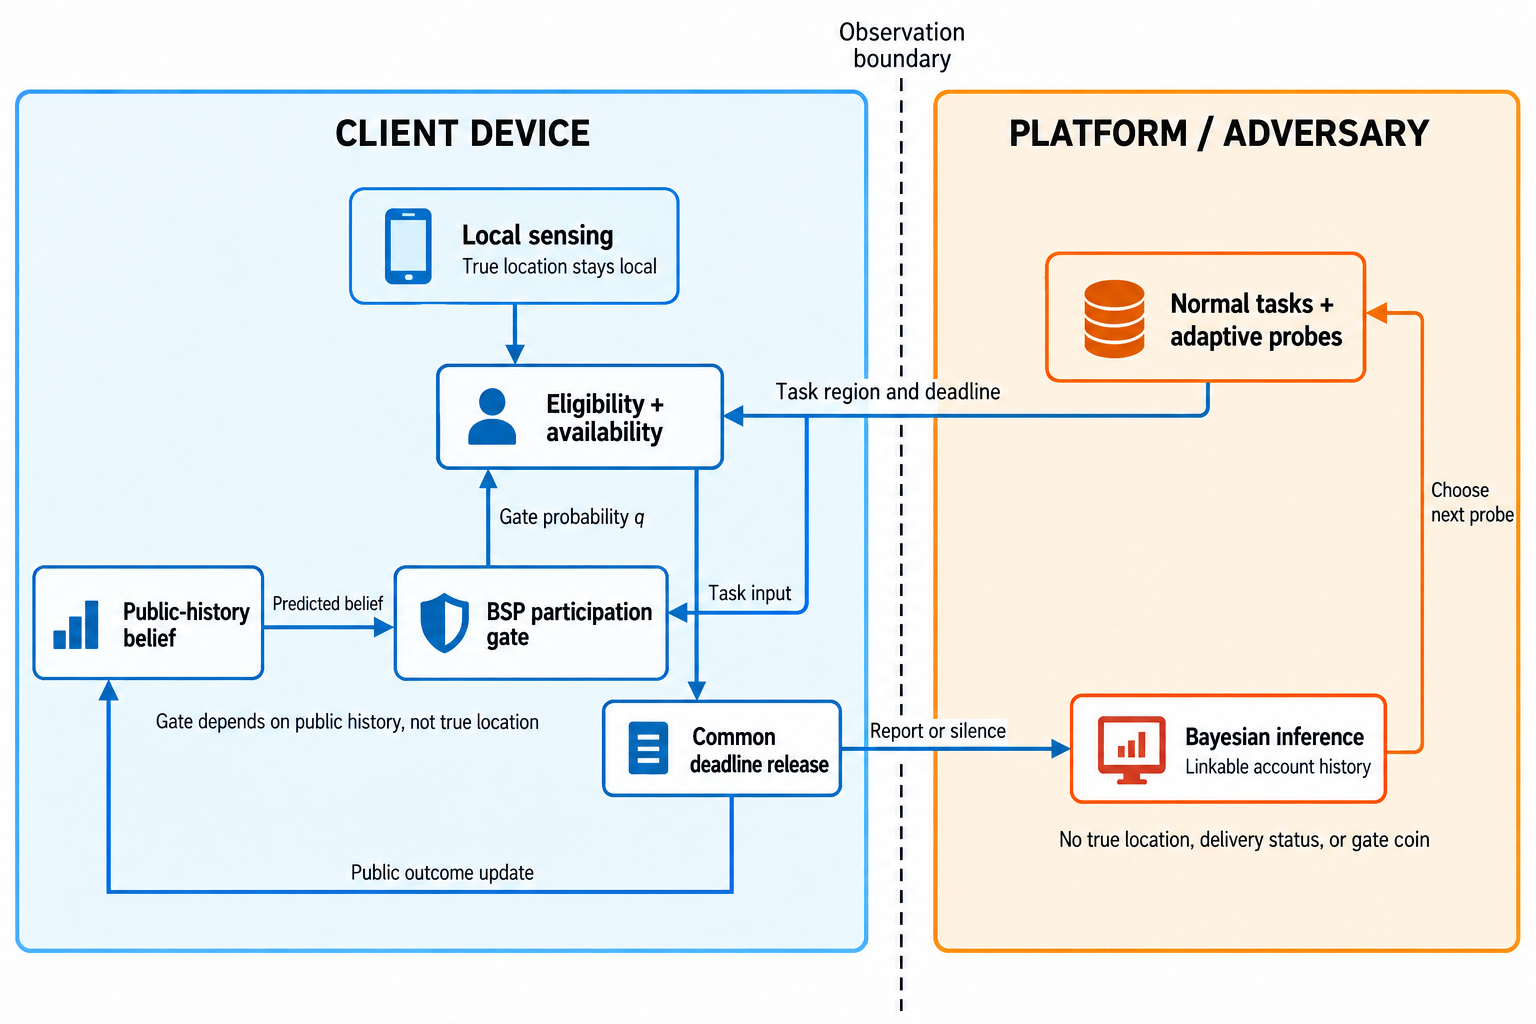
\includegraphics[width=\linewidth]{figures/system_architecture.png}
\caption{System architecture and observation boundary. A linkable account produces a truthful report or silence at a common deadline. The platform selects normal tasks and adaptive probes from public history. The BSP gate uses predicted belief and task metadata; true location is used locally for eligibility. The platform does not directly observe true location, task-delivery status, or the gate coin. This is a conceptual, image-model-generated schematic, not an experimental result.}
\label{fig:architecture}
\end{figure}
\subsection{Tasks and private state}
Let $X_t\in\mathcal X$ denote a user's location cell at the sampling instant in slot $t$, where $|\mathcal X|=N$. A task specifies a public region $S_t\subseteq\mathcal X$, a sampling slot, and a deadline. A valid report requires an observation collected inside $S_t$ at that sampling instant and submitted by the deadline. Receiving or accepting a task is not sufficient. All timely reports are released at the slot boundary, giving a fixed one-slot reporting delay in the simulator.

Let $D_t,W_t,L_t$ denote successful delivery, willingness to participate, and timely completion. In the baseline model these are independent Bernoulli variables, independent of location conditional on public history, with product probability $\alpha_t$. The filter additionally samples $G_t\sim\mathrm{Bernoulli}(q_t)$ independently. The only published outcome is
\begin{equation}
 Y_t=\ind\{X_t\in S_t\}D_tW_tL_tG_t\in\{0,1\}.
 \label{eq:output}
\end{equation}
Here $Y_t=0$ means that no valid report appeared by the deadline. There are no separate acknowledgments of delivery, online status, refusal, or filter rejection. Reports do not disclose additional measurement content in this model. If such content, network metadata, or fine-grained submission times are visible, the observation channel must be extended before applying the guarantee.

This design represents opportunistic sampling at a specified instant, not continuous movement toward a newly assigned destination. Users do not change their paths in response to tasks. The simulated normal task stream is public and exogenous. Probe tasks share the same completion requirements and cannot be recognized by the client as probes.

\subsection{Attacker knowledge and capabilities}
The platform links outcomes to an account, knows the task regions, deadlines, filtering algorithm, and its parameters, and retains the account's public history. At designated probe slots, it may choose a task region from a finite public library using that history. It does not observe the simulator's actual location, future trajectory, delivery draws, willingness, or deadline-success draws. A prior-only estimator receives no outcomes. A fixed attack uses independently selected regions. An adaptive attack selects the next probe to maximize one-step mutual information under its current belief and the known gate. This greedy attack is a reproducible adversary, not a proof of optimal sequential inference or task selection.

The principal analytical model assumes that client and attacker use the same correct mobility and observation models. The main replay experiment relaxes correctness: both use the same approximate model. Separate stress tests give the attacker the correct generating probabilities while leaving the client's probabilities misspecified. Auxiliary information about an individual's home, routines, network attachment, or other accounts is outside the main model.

\subsection{Bayesian observation channel}
Let $b_t(i)=\Pr(X_t=i\mid H_{t-1},S_t)$ be the predicted belief before the current output, and abbreviate $b=b_t$, $h_i=\alpha_t\ind\{i\in S_t\}$, and $m=\sum_i b_i h_i$. A gate is a deterministic function of public history and the current task; its random coin is private. For $q>0$ and $m>0$, the report posterior is
\begin{equation}
 b_i^+=\frac{b_i h_i}{m}.
 \label{eq:positive}
\end{equation}
For a positive-probability silence branch, it is
\begin{equation}
 b_i^-=\frac{b_i(1-qh_i)}{1-qm}.
 \label{eq:silence}
\end{equation}
Zero-probability branches impose no condition. For example, when $q=0$, silence leaves the predicted belief unchanged. With $\alpha_t<1$, silence generally preserves positive probability inside $S_t$. Between slots, a public transition matrix predicts the next location belief.

We evaluate posterior concentration through $\|b\|_\infty$, as well as attack hit rate, error, log loss, and calibration. A count of plausible cells alone is not a probability bound. A posterior with many nonzero entries can still place nearly all probability on one cell.

\section{Branch-safe participation}
\label{sec:method}
\subsection{Feasible gate and interpretation}
Fix a desired posterior threshold $\rho$ and set $c=\max\{\rho,\|b\|_\infty\}$. The local objective is to maximize $q\in[0,1]$ subject to $\|b^y\|_\infty\le c$ for each positive-probability output $y$. Using $c$ prevents a request from being infeasible solely because the predicted belief already exceeds $\rho$. In that situation the rule prevents additional peak concentration relative to the current belief; it cannot restore a previously violated absolute threshold.

\begin{proposition}[Maximal scalar gate]
If $m>0$ and $\max_i b_i h_i/m>c$, the only feasible gate is $q^*=0$. Otherwise, define $d_i=cm-b_i h_i$. Then the maximal feasible scalar gate is
\begin{equation}
 q^*=\min\left\{1,\min_{i:d_i>0}\frac{c-b_i}{d_i}\right\},
 \label{eq:gate}
\end{equation}
where an empty inner minimum is $+\infty$. When $m=0$, this expression gives $q^*=1$ and the output is uninformative.
\end{proposition}
\begin{proof}
For every $q>0$ with $m>0$, Eq.~\eqref{eq:positive} is independent of $q$. If its peak exceeds $c$, no positive gate can satisfy the report constraint. Otherwise only the silence constraints remain. For a nonzero silence probability, Eq.~\eqref{eq:silence} is at most $c$ exactly when
\begin{equation}
 q(cm-b_i h_i)\le c-b_i\quad\text{for all }i.
\end{equation}
The right side is nonnegative. A nonpositive coefficient on the left imposes no upper bound on $q$; a positive coefficient gives the bound in Eq.~\eqref{eq:gate}. Their intersection with $[0,1]$ yields the stated maximum. If silence has zero probability, the corresponding constraint is vacuous and the same expression admits $q=1$. Finally, $q=0$ is always feasible because the resulting posterior equals $b$.
\end{proof}

The calculation takes $O(N)$ time for one task and stores an $N$-cell belief. Maximizing $q$ maximizes the current expected completion probability $qm$ within this scalar family. It does not optimize the utility of future tasks. In particular, consuming available posterior concentration now can restrict later participation. A nonmyopic scheduler or a mechanism whose gate depends on private location would be a different optimization problem.

\begin{corollary}[Conditional sequential cap]
Suppose the initial belief has peak at most $\rho$, the declared models are correct, all public signals are represented by Eq.~\eqref{eq:output}, and every location transition is doubly stochastic. Then BSP maintains posterior peak at most $\rho$ after every output, including under adaptive task selection measurable from public history.
\end{corollary}
\begin{proof}
A doubly stochastic transition makes each predicted probability a convex combination of previous probabilities, so prediction cannot increase the maximum. The proposition bounds both possible observation branches by $\rho$. Induction over slots proves the result. Given the public history, the attacker's adaptive task choice supplies no additional private-state information under the stated measurability assumption.
\end{proof}

The corollary applies to the declared posterior, and to an attacker's posterior only when the knowledge and model assumptions coincide. It is not robust to arbitrary prior knowledge, location-dependent availability, undisclosed outputs, or an attacker with a more accurate mobility model. A reflecting symmetric grid walk satisfies the transition condition. A general learned human-mobility transition need not do so.

\subsection{Finite-model robust extension}
\label{sec:robust}
The informed-attacker failure motivates an explicit, limited form of model uncertainty rather than a distribution-free claim. Let $\mathcal M=\{M_1,\ldots,M_K\}$ be a finite public ambiguity set fixed independently of the current private state. Model $M_k$ maintains its own public-history belief $b_t^{(k)}$, transition rule, and availability probability $\alpha_t^{(k)}$. For the current task, let $q_k^*$ be the maximal BSP gate from Proposition~1 using that model and $c_k=\max\{\rho,\|b_t^{(k)}\|_\infty\}$. Robust BSP (R-BSP) uses
\begin{equation}
 q_R^*=\min_{1\le k\le K} q_k^*.
 \label{eq:robust-gate}
\end{equation}
All member beliefs are updated from the same public task and report/silence history; none receives the true location or the gate coin.

\begin{proposition}[Maximal common finite-model gate]
Within the class of one scalar gate shared by all models, Eq.~\eqref{eq:robust-gate} is the largest $q\in[0,1]$ for which both positive-probability output branches satisfy $\|b_{t,k}^{y}(q)\|_\infty\le c_k$ for every $M_k\in\mathcal M$.
\end{proposition}
\begin{proof}
For each fixed model, Proposition~1 gives the complete feasible scalar set as the interval $[0,q_k^*]$: if the positive branch is infeasible then $q_k^*=0$; otherwise the silence inequalities supply only upper bounds on $q$. Requiring all models simultaneously intersects these intervals, giving $[0,\min_k q_k^*]$. Its right endpoint is therefore the maximal common gate.
\end{proof}

R-BSP costs $O(KN)$ per task when each member uses the $N$-cell implementation above. If an attacker's exact Bayesian model is one member of $\mathcal M$, the corresponding branch constraint applies to that attacker as well; under the transition conditions of the corollary, its model-specific sequential cap is preserved. This statement does not cover an attacker outside the ambiguity set, unmodeled observations, or arbitrary auxiliary information. Enlarging $\mathcal M$ can only weakly decrease the feasible gate, so model-set construction is itself a privacy--utility design choice.

\subsection{Why reports and silence both matter}
Equation~\eqref{eq:positive} gives a basic limitation: reducing a scalar participation probability does not weaken the conditional evidence of a report that actually occurs. Thinning reduces how often that report occurs. If a task identifies a single cell, every truthful successful report identifies that cell regardless of how small $q$ is. BSP must reject tasks whose positive branch violates the cap.

Checking only successful reports is nevertheless insufficient. Consider $b=(0.2,0.2,0.2,0.4)$, $S=\{1,2,3\}$, $\alpha=0.9$, and $c=0.4$. The report posterior has peak $1/3$, so a success-only rule allows $q=1$. After silence, the fourth cell has probability $0.4/0.46\approx0.870$, violating the cap. BSP instead sets $q=0$. This example also illustrates a potential utility cost when the current belief already has a cell at the cap.

There is a separate support obstruction to pure location differential privacy. For any proper region and any nonzero truthful reporting probability inside it, the report event has positive probability inside and zero probability outside. No finite multiplicative likelihood-ratio bound can hold between those two states for that event. This elementary observation does not rule out other privacy definitions, altered report semantics, or mechanisms with false positives. It explains why the present filter must not be described as a differentially private coordinate-release mechanism.

\subsection{Execution procedure}
Figure~\ref{fig:workflow} summarizes the two-branch check and the illustrative silence calculation.
\begin{figure}[tbp]
\centering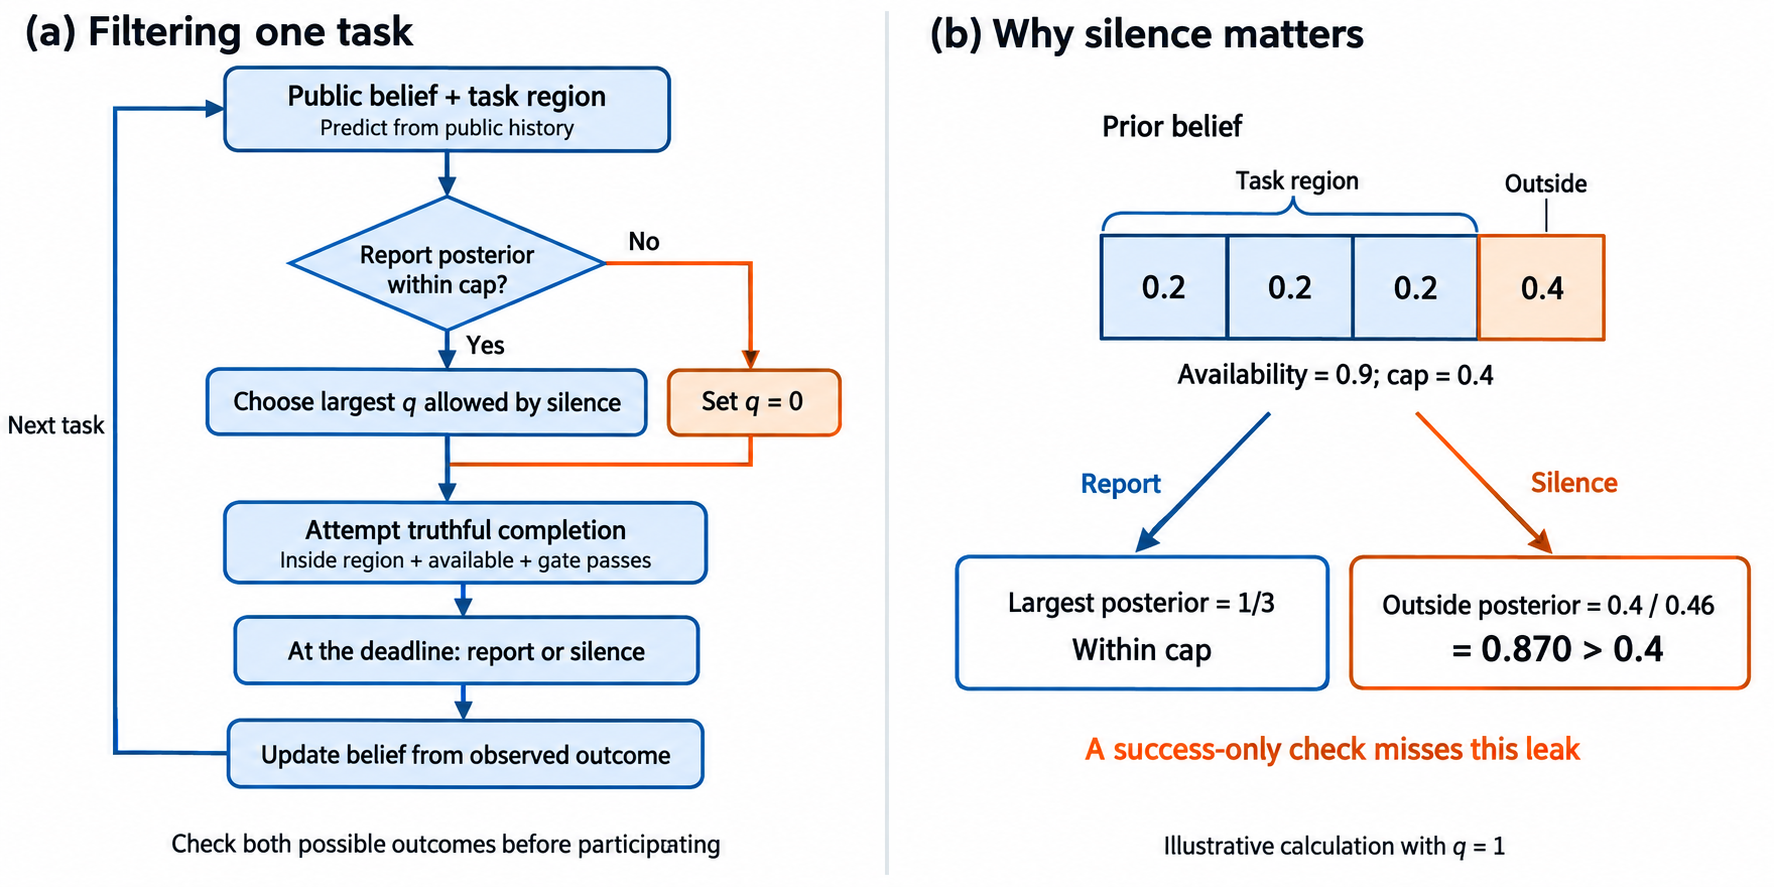
\includegraphics[width=\linewidth]{figures/bsp_workflow.png}
\caption{BSP workflow and a four-state analytical example. Both positive-probability branches must satisfy the cap. With $q=0$ the gate never passes and only silence can occur; a zero-probability report branch needs no check. In panel (b), a success-only rule accepts $q=1$, although silence raises the outside-cell posterior to about 0.870. BSP sets $q=0$ for this example. Image-model-generated schematic; numbers follow the stated calculation, not simulated measurements.}
\label{fig:workflow}
\end{figure}
At each slot the client predicts its belief, reads the public region and deadline, and computes $q^*$. It samples the gate independently of its location, attempts the task only if permitted, and releases any valid report at the common deadline. The public posterior is updated using either Eq.~\eqref{eq:positive} or Eq.~\eqref{eq:silence}. The platform can reproduce $q^*$ from the same declared model and history without receiving the gate coin. No extra refusal message is sent.

The implementation uses half-open rectangles. It rejects repeated task identifiers, checks agreement between task and observation identifiers and sampling slots, and rejects task deadlines preceding their sampling slots. It does not implement arrival-time validation for late network messages; timely completion is represented by the Bernoulli variable in Eq.~\eqref{eq:output}. True locations are consulted only by the response simulator and evaluation metrics. Archived evaluation logs contain ground truth for auditing, but the attack receives only public tasks, outcomes, model parameters, and the gate determined by public history.

\section{Experimental design}
\label{sec:experiments}
\subsection{Data and task generation}
The evaluation uses Python event simulation, NumPy, and local algorithm timing. It requires no sensing hardware or paid cloud service. The main grid has $8\times8$ cells and each trajectory contains 48 slots. Synthetic mobility is static, a reflecting random walk with move-attempt probability $0.3$, or periodic movement back and forth along a row. The first two start uniformly. The periodic condition uses a random row and phase; its initial distribution and temporal dependence are intentionally not represented by the attacker's uniform-prior random-walk model. Synthetic cells have a nominal width of 1 km for distance reporting.

GeoLife~\cite{geolife2009,geolife2008,geolife2010}\footnote{Microsoft Research, GeoLife GPS Trajectories, archive version 1.3: \url{https://www.microsoft.com/en-us/download/details.aspx?id=52367}. The download page requests the three original dataset-related citations.} provides observed locations for replay, not task logs. Tasks, delivery, participation, and completion remain simulated. For each user, we select the first lexicographically ordered file containing 48 consecutive minute bins with samples in latitude $[39.8,40.1)$ and longitude $[116.2,116.6)$. We take the first in-bounds sample in each minute, without interpolating gaps or joining files. This retains 107 of 182 users; 75 have no qualifying window. User ID modulo five assigns 23 development, 17 validation, and 67 test users, each contributing one window. Test users are excluded from mobility-parameter and PRIVIC-channel fitting. The later thinning-grid extension and policy-envelope selection use test results and are exploratory analyses, not independent validation of a selected policy. The validation split was reserved but not used to select those envelopes.

The development fraction of consecutive samples changing grid cell is $0.0508788$, used as the approximate replay walk parameter. Jump distances and directions are not fitted. Boundary reflection also means that a cell-change fraction is only a proxy for a move-attempt probability. This is an approximate mobility model, not a validated human-movement predictor. The geographic cells are approximately 4.17 km north--south and 4.27 km east--west, so the experiment concerns coarse cell inference rather than address recovery. At this resolution, \ReplayStaticWindows/67 test windows remain in one cell throughout and the median window visits \ReplayMedianCells\ distinct cells. A post-review diagnostic additionally fits a fixed no-output predictor using the most frequent cell among development positions only, with ties averaged uniformly. Test positions evaluate that frozen predictor; they do not select its cell. This diagnostic does not change or rerun the original uniform-prior attacks.

The main public library contains 152 rectangles: squares at several widths and horizontal or vertical prefix/suffix strips. Normal task regions are sampled uniformly. A shared Bernoulli schedule chooses a normal task with probability $0.75$ and a probe otherwise. Delivery, willingness, and timely-completion probabilities are $0.9$, $0.8$, and $0.9$, giving $\alpha=0.648$. Sampling occurs at the slot's specified instant and reports are released at its deadline. Varying timely-completion probability does not simulate continuous movement within variable-length acquisition windows.

\subsection{Policies and fair comparison}
The main policy grid contains no filtering; random participation probabilities $0.15,0.3,0.5,0.7$; periodic admission every $2,4,8$ slots; admission of rectangles aligned to blocks of side $2$ or $4$; BSP thresholds $0.05,0.1,0.2,0.4$; and a success-only ablation at $0.1$. The aligned-grid policy rejects nonaligned tasks. It does not enlarge task regions, forge completions, or implement an anonymity protocol.

A later exploratory extension adds a KL branch filter at $\kappa=0.25,0.5,1,2$ nats. This adaptation of Bayesian privacy~\cite{bayesian} approximates the largest scalar $q$ satisfying $D_{\mathrm{KL}}(b^y\|b)\le\kappa$ for both positive-probability branches. For positive prior region mass and nonzero availability, the report divergence is $-\log\Pr_b(S)$; silence divergence reduces to a binary region partition and is solved with 30 bisection steps. Zero-mass candidate regions use $q=0$ in the implementation; their output is uninformative for any gate under the declared prior. It limits each update relative to its current prior, not cumulative session KL or an absolute posterior maximum. It is not a reproduction of the published economic mechanism.

For each trajectory and seed, policies share the normal tasks and all exogenous random draws. Fixed and adaptive attacks are rerun for every main policy; adaptive probes may therefore differ. The greedy attack searches the library for maximal expected information under the known gate. There is one probe per probe slot. Probe completions contribute observations but do not count as normal-task utility. A pilot's fixed normal/probe schedule was confounded with periodic admission; the main run corrects this by using an independent shared random schedule. Pilot results are retained but excluded.

\subsection{Recent optimization-based comparators}
\label{sec:recentmethods}
\paragraph{PML-T (TIFS 2024 constraint specialization)}
PML bounds the maximum posterior-to-prior likelihood ratio for each output. Lemma 1 of Grosse et al.~\cite{pml2024} expresses this as linear constraints on a stochastic channel. We specialize those constraints to truthful binary completion and maximize its expected probability. Write $l_i=\Pr(Y=1\mid X=i)$ and $m=\sum_i b_i l_i$. The linear program is
\begin{equation}
\begin{aligned}
 \max_l\quad & m,\\
 \text{subject to}\quad &0\le l_i\le\alpha\ind\{i\in S\},\\
 &l_i\le e^\epsilon m,\qquad 1-l_i\le e^\epsilon(1-m),\quad b_i>0.
\end{aligned}
\label{eq:pml}
\end{equation}
If $M=\sum_{i\in S}b_i<e^{-\epsilon}$, a nonzero report is infeasible: summing the report constraint over $S$ gives $m\le e^\epsilon M m$. If $e^{-\epsilon}\le M<1$, the outside-state silence constraint and the availability bound give $m\le\min(\alpha M,1-e^{-\epsilon})$. Constant likelihood $l_i=\alpha q$ inside $S$, with $q=\min\{1,(1-e^{-\epsilon})/(\alpha M)\}$, attains their minimum for $\alpha>0$. If $\alpha=0$, every gate has zero completion probability. When $M=1$, $q=1$ is feasible; when $M=0$, the gate does not affect the output. Thus this specialization is exactly optimal for current completion even among location-dependent gates. We verify it against an independent general linear program over 100 random priors. This is our binary-channel instantiation of the published constraints, not a reproduction of the paper's general-output vertex-enumeration experiment. The tested $\epsilon$ values are $0.025,0.05,0.1,0.25,0.5,1,2,4,8$ nats per update.

\paragraph{PRIVIC-T (PoPETs 2024 mechanism with task adaptation)}
We implement the paper's incremental BA--IBU loop and final generalized IBU (GIBU), followed by BA~\cite{privic2024}. BA minimizes mutual information plus $\beta$ times expected spatial distortion. Training uses only development locations: synthetic seeds 4000--4019 or the 23 development replay users. Eight shuffled collection batches release noisy locations through their current channels; only those noisy counts enter IBU/GIBU. The training seed is 42024. The resulting $64\times64$ channel $C$ is frozen before testing. We report all $\beta\in\{0,0.1,0.3,1,3,10\}$, where zero is an independent-output boundary control and distances are in cells. BA/IBU recurrences match the author code on fixed-iteration checks; the paper's final GIBU step is also implemented. Iterations stop at maximum component change below $10^{-8}$ or 100,000 iterations, with residuals and limit hits archived.

To connect the location mechanism to a valid-task interface, the client admits a task when a privately sampled surrogate $Z\sim C_{X,:}$ lies inside its region, while still requiring the true location to be inside. The surrogate is not transmitted. Consequently the report likelihood is
\begin{equation}
 l_i=\alpha\ind\{i\in S\}\sum_{z\in S}C_{iz}.
\label{eq:privic}
\end{equation}
The simulator samples the equivalent Bernoulli event. Both the attack's probe objective and its report/silence update use the entire public likelihood vector; neither receives the true-state-indexed gate probability. This task adapter is explicitly ours. Checking true eligibility after perturbation is not post-processing of $Z$ alone, so PRIVIC's original geo-indistinguishability guarantee does not transfer. Likewise, task completion is different from the original location-distortion or population-estimation utility. We label the result PRIVIC-T to keep that distinction visible.

The initial extension adds 60 conditions and 4,605 trajectory executions. Because its PRIVIC-T settings did not cover retention 0.5 in several scenarios, we subsequently add public random thinning factors $\gamma=0.25,0.5,0.75$ for every PRIVIC-T setting, multiplying Eq.~\eqref{eq:privic} by $\gamma$. These 72 additional conditions contribute 5,526 executions, while retaining the original $\gamma=1$ cases. No training channel changes. All methods use the same test users, normal tasks, exogenous randomness, and clustering, with adaptive probes regenerated separately for each setting. The two published mechanisms offer optimized constraints or rate--distortion objectives; simple policies remain diagnostic controls. The initial grid was fixed before its test run; the thinning grid was fixed after observing the initial coverage gap. This is an explicitly exploratory extension.

All 24 final BA channels reach the declared iteration-change tolerance. Seven final GIBU fits reach the iteration limit; their finite-iteration estimates are retained and identified. A concavity-based gradient bound on the mean log-likelihood optimization gap is at most $1.06\times10^{-5}$ nats per sample across all final GIBU fits. This numerical bound concerns the fitted objective, not recovery of the true population distribution. Intermediate-loop residuals and limit hits are also archived.

\subsection{Metrics and inference units}
MAP cell hit rate and Euclidean grid error average over slots, resolving maximum-posterior ties uniformly in expectation. Replay error also uses a local latitude/longitude distance scale. We record posterior peak, entropy, log loss, 95\% credible-set size and coverage, and ten-bin calibration error. Credible sets include descending-probability cells until cumulative mass reaches 0.95, breaking probability ties by cell index. MAP ties use numerical tolerances of $10^{-10}$ relative and $10^{-14}$ absolute. Discreteness and model mismatch prevent interpreting nominal mass as a guaranteed empirical coverage rate.

Legitimate opportunity retention is
\begin{equation}
 U=\frac{\text{valid normal-task completions}}{\text{eligible normal tasks externally completable without filtering}}.
 \label{eq:utility}
\end{equation}
The denominator uses the same delivery, willingness, and deadline draws as the numerator and excludes only the gate. Table~\ref{tab:main} additionally reports raw completion, defined as summed valid completions divided by all normal tasks, including those for which the user was outside the region or externally unavailable. This pooled ratio differs from averaging per-user completion fractions. A descriptive post-review analysis stratifies the executed BSP $\rho=0.1$ logs into regions of 1--8, 9--31, and 32--64 cells; it does not characterize policy-envelope mixtures. We also save coverage of opportunity cells, unit reward per completion, delay, and real gate execution time. Reward is not economic welfare. Reporting delay is one slot by construction, not measured network latency.

The main run has 120 conditions and 9,210 trajectory executions: 20 independent synthetic seeds, four users per seed, or 67 replay users per condition. The KL extension adds 16 conditions and 1,228 executions. These are repeated evaluations of shared trajectories, not 10,438 distinct people. Risk estimates average users within seed clusters; retention is a ratio of summed completions to summed opportunities. We use 1,000 percentile-bootstrap resamples, clustering by synthetic seed or replay user. Repeat counts were a computationally modest design choice, not a formal power calculation.

Utility-adjusted comparisons linearly interpolate observed curves at retention 0.5 and 0.7, without extrapolation. Paired resampling uses the same cluster indices across policies. We report an interval only when original curves overlap and at least 95\% of resamples retain overlap. These are exploratory interpolations, not independently deployed policies tested at exactly matched completion rates. Intervals are pointwise without multiplicity correction and do not quantify generalization to unsampled populations.

For the recent-method extension, we strengthen the comparison by using each method's lower convex envelope over \emph{all} tested settings, rather than connecting dominated parameter points. An envelope segment describes expected performance when a setting is selected for an entire trajectory and revealed to the attacker before that trajectory. Normal-task opportunity denominators are shared across settings, so expected completion retention and mean risk mix linearly. We recompute the envelope in every paired bootstrap sample and apply the same overlap rule. These are exploratory envelopes selected using test results, not independently validated tuned policies; selection and the finite grid limit inferential interpretation. Their intervals are conditional on the fixed development sample and fitted PRIVIC channels. They exclude training-noise variability and do not refit BA/IBU/GIBU; different thinning factors share the same channel. Raw points and ordinary adjacent-point interpolations are retained separately. The no-output replay diagnostic uses 1,000 user-bootstrap resamples conditional on its fixed development-fitted predictor, with seed 170926.

\subsection{Sensitivity and stronger knowledge}
The sensitivity run contains 72 conditions, ten independent seeds with four users each, and 2,880 executions. It varies true mobility, delivery, willingness, timely completion, assumed availability and mobility, normal-task fraction, grid side, and ideal history-reset period. Each condition compares no filtering, random participation at 0.5, and BSP at 0.1. Resets every 1, 4, or 12 slots erase account history; they do not implement unlinkable rotating identities. Changing grid size also changes the inference target and task library.

Twelve additional exploratory conditions, totaling 480 executions, give the attacker correct generating probabilities while the client uses a wrong probability. The true walk and availability probabilities are $v=0.3$ and $\alpha=0.648$; the client uses $\widehat\alpha=0.3$ or $0.9$, or $\widehat v=0.05$ or $0.8$. The attacker maintains its own belief and chooses probes using that belief and the client's public gate. It receives no true locations or future trajectory. This is a stronger test than giving both parties the same incorrect model.

After observing these nominal-model failures, we add a separately recorded, post-hoc R-BSP stress test rather than reclassifying it as pre-specified evidence. The decision to form a finite ambiguity set is post-hoc, but its parameter levels are inherited from the earlier sensitivity and informed-attacker configurations rather than selected from R-BSP outcomes: the $3\times3$ grid uses $v\in\{0.05,0.3,0.8\}$ and $\alpha\in\{0.3,0.648,0.9\}$. Twenty new synthetic seeds (3000--3019), four users per seed, and 48 slots evaluate nominal, low/high assumed $\alpha$, and low/high assumed $v$ for BSP and R-BSP at $\rho\in\{0.05,0.1,0.2,0.4\}$, yielding 40 conditions and 3,200 trajectory executions. The evaluator's informed attacker uses the generating model $v=0.3,\alpha=0.648$, which is deliberately included in the R-BSP set. The primary stress endpoint is the fraction of slots where the attacker's posterior after an output exceeds its own pre-output local cap $\max\{\rho,\|b_t^{A}\|_\infty\}$. Because the ambiguity grid was designed in response to the earlier failure, this experiment is mechanism validation and cost characterization, not independent confirmation.

We then add a second post-hoc boundary characterization on 20 further synthetic seeds (4000--4019), again with four users and 48 slots. It keeps the nine-member R-BSP set fixed and evaluates four correct attacker/generating models that are not members of that set: $\alpha=0.50$ and $v=0.50$ lie between enumerated values, whereas $\alpha=0.98$ and $v=0.95$ lie beyond the set's upper ranges. Nominal BSP and R-BSP are compared only at $\rho=0.1$, giving eight conditions and 640 trajectories. This run is designed to probe the boundary of the finite-set claim, not to enlarge the theorem after seeing the outcomes.

\section{Results}
\label{sec:results}
\subsection{Information beyond the specified uniform prior}
A uniform prior gives expected MAP hit rate $1/64\approx1.56\%$ when ties are randomized uniformly. Under adaptive probes with no filtering, hit rates are \StaticNoneHit\% for static users, \WalkNoneHit\% for random walks, \CommuteNoneHit\% for periodic mobility, and \GeolifeNoneHit\% for replay. Outputs improve the specified uniform-prior estimator in these task processes. This demonstrates a possible mechanism under declared assumptions, not its observed prevalence on a deployed platform or the incremental leakage over every plausible prior.

Table~\ref{tab:prior-diagnostic} shows why the prior qualification matters for replay. The most frequent development cell, index 34, has development mass \PopulationPriorPeak\%; always predicting it attains \PopulationPriorHit\% test accuracy without task outputs. This exceeds the uniform-prior attack's \GeolifeBspHit\% accuracy under BSP $\rho=0.1$. An observer with the development statistics could choose that no-output predictor instead, so the latter number is not an upper bound on its attainable accuracy. The diagnostic is not a rerun of a stronger adaptive attack and does not replace the original paired comparison. Nor does it refute the conditional sequential cap: this nonuniform initial peak already exceeds 0.1. A population-prior adaptive evaluation would require declaring a different belief model and interpreting the local cap accordingly.

\begin{table}[tbp]
\centering\small
\caption{No-output replay diagnostics on 67 test users with 48 slots each. The modal cell is fitted only on 23 development users. Its pointwise interval resamples test users and conditions on that fixed predictor; the uniform row is an exact randomized-tie expectation. Neither row observes task outcomes.}
\label{tab:prior-diagnostic}\begin{tabular}{lrr}
\toprule
No-output predictor & Hit (\%) & 95\% interval \\
\midrule
Uniform random cell & 1.56 & Exact expectation \\
Development modal cell & 25.75 & [17.88, 34.83] \\
\bottomrule
\end{tabular}

\end{table}

\begin{figure}[tbp]
\centering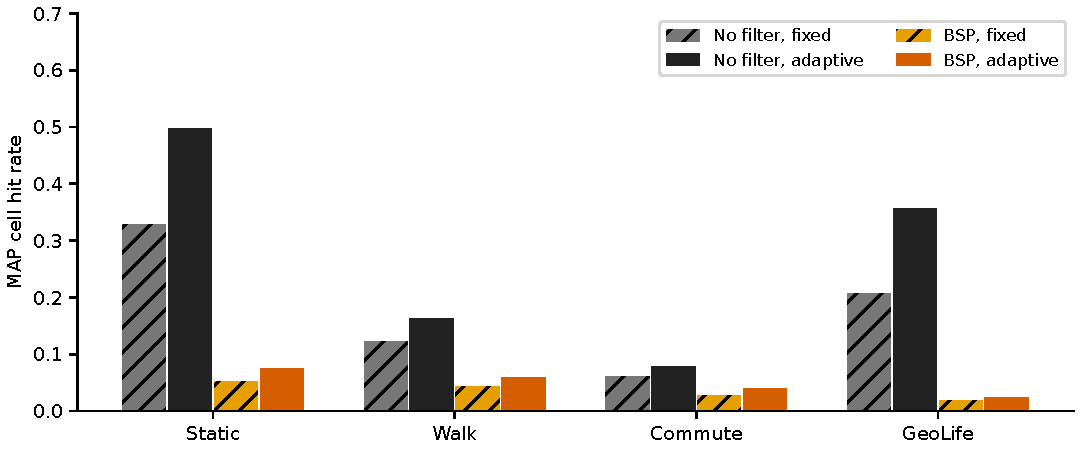
\includegraphics[width=\linewidth]{attacks.pdf}
\caption{Fixed and defense-aware adaptive probes. Each main condition has 20 synthetic seed clusters or 67 replay users. The adaptive objective is expected information under the model, not realized MAP accuracy; it need not improve every empirical metric.}
\label{fig:attacks}
\end{figure}

\subsection{Participation and inference}
Figure~\ref{fig:tradeoff} shows all adaptive policy thresholds, including the exploratory KL extension. Table~\ref{tab:main} reports representative executed conditions. At $\rho=0.1$, BSP retains \StaticBspRetention\%, \WalkBspRetention\%, \CommuteBspRetention\%, and \GeolifeBspRetention\% of normal-task opportunities, with hit rates \StaticBspHit\%, \WalkBspHit\%, \CommuteBspHit\%, and \GeolifeBspHit\%, respectively. These are nonzero completions under the current region library and equal-reward convention; they do not establish preservation of fine-region sensing service.

The task-size breakdown in Table~\ref{tab:task-area} shows that \LargeTaskShareMin--\LargeTaskShareMax\% of these completions come from regions covering at least 32 of 64 cells. None of the 1--8-cell opportunities is completed. This matches the support restriction: at posterior cap 0.1, any permitted positive report needs at least ten positive-probability cells. Raw completion over all normal tasks is only \RawCompletionMin--\RawCompletionMax\%, partly because many tasks are ineligible even before filtering. The approximately one-half opportunity retention therefore refers to a restricted denominator and favors large-region tasks. This descriptive breakdown concerns the executed $\rho=0.1$ conditions, not the matched-retention envelopes.

\begin{figure}[tbp]
\centering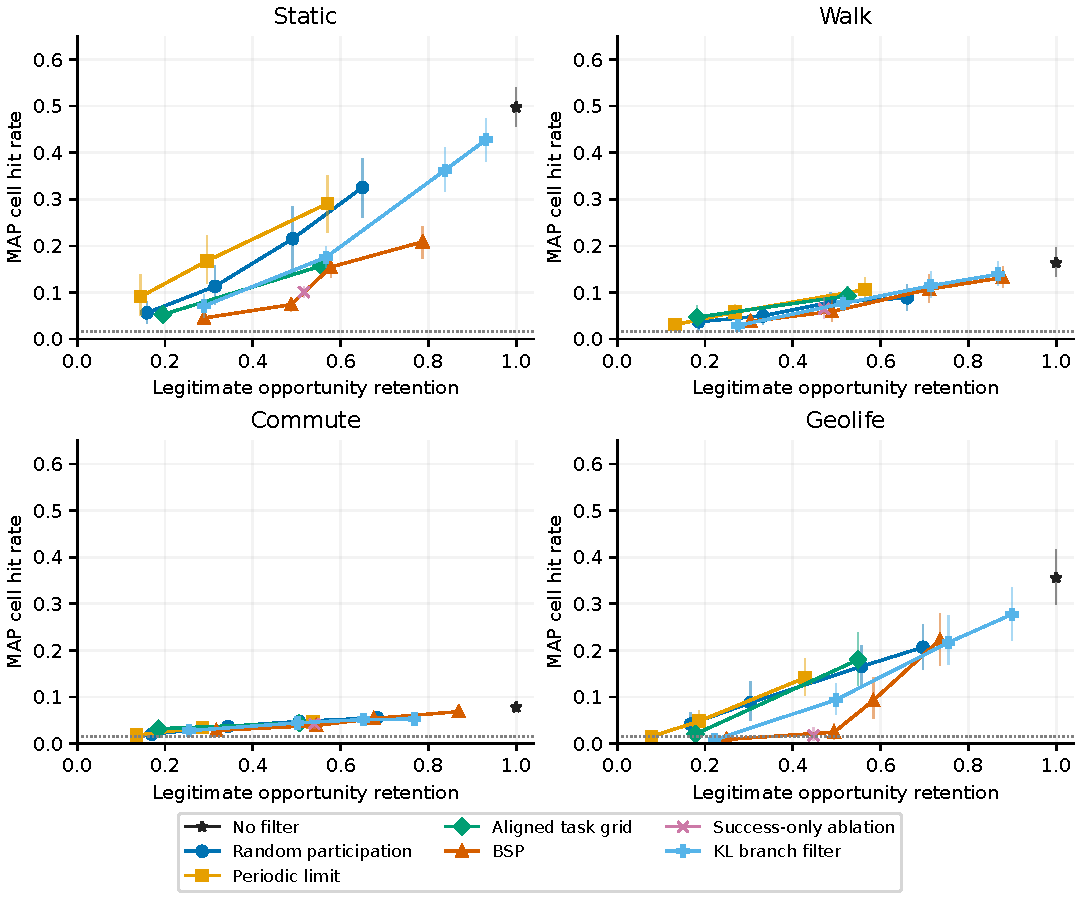
\includegraphics[width=\linewidth]{tradeoff.pdf}
\caption{Opportunity retention and MAP hit rate under adaptive probes. Symbols are executed settings; connecting lines are visual guides. Error bars are pointwise 95\% cluster-bootstrap intervals for hit rate, from 20 synthetic seed clusters or 67 users. The dotted line is the uniform-prior rate. Higher retention and lower hit rate are preferred.}
\label{fig:tradeoff}
\end{figure}
\begin{table}[tbp]
\centering\footnotesize
\caption{Representative executed adaptive conditions. Retention uses Eq.~\eqref{eq:utility}; raw completion divides summed completions by all normal tasks, including ineligible tasks. Both are fractions. Error is in grid cells, whose geographic sizes differ across synthetic and replay scenarios. Complete estimates and intervals are saved as CSV.}
\label{tab:main}\input{main_table_revision}
\end{table}

At interpolated retention 0.5, BSP minus random participation has a hit-rate difference of $-13.62$ percentage points for static users, with pointwise 95\% interval $[-20.02,-7.51]$, and $-11.91$ points for replay, with interval $[-16.32,-6.07]$. Table~\ref{tab:matched} also shows lower risks than the KL adaptation in those two scenarios. In contrast, walk and periodic comparisons against both random participation and KL have intervals containing zero. They do not establish a consistent advantage.

Several coarse-grid and periodic-limit comparisons have insufficient utility overlap for stable interpolation. In replay, periodic-limit settings do not bracket retention 0.5; we make no matched claim there. Lower risk at a substantially lower completion level is not evidence of a superior trade-off.

\begin{table}[tbp]
\centering\small
\caption{Exploratory interpolation at retention 0.5. Hit rates and differences are in percentage points. Paired cluster-bootstrap intervals are pointwise. All displayed comparisons have 1,000 valid overlapping resamples.}
\label{tab:matched}\begin{tabular}{llrrr}
\toprule
Scenario & Comparator & BSP hit & Other hit & Difference [95\% CI] \\
\midrule
Static & Random & 8.52 & 22.15 & -13.62 [-20.02, -7.51] \\
Static & KL & 8.52 & 15.03 & -6.51 [-9.42, -3.25] \\
Walk & Random & 6.14 & 7.95 & -1.81 [-4.55, +2.00] \\
Walk & KL & 6.14 & 7.33 & -1.20 [-3.74, +2.15] \\
Commute & Random & 3.67 & 4.72 & -1.05 [-2.08, +0.07] \\
Commute & KL & 3.67 & 4.43 & -0.76 [-1.52, +0.04] \\
Geolife & Random & 2.89 & 14.80 & -11.91 [-16.32, -6.07] \\
Geolife & KL & 2.89 & 9.47 & -6.59 [-10.03, -2.01] \\
\bottomrule
\end{tabular}
\end{table}

\subsection{Comparison with 2024 mechanisms}
Figure~\ref{fig:recent} and Table~\ref{tab:recent} use the strengthened policy envelopes, including the additional PRIVIC-T thinning settings. At retention 0.5, BSP's static hit-rate advantage is 8.77 percentage points over PML-T and 10.62 points over PRIVIC-T; the pointwise exploratory intervals exclude zero. For replay, the PML-T difference is $-7.30$ points, whereas the PRIVIC-T difference is $-4.28$ points with an interval containing zero. In the walk scenario, PRIVIC-T has the lower point estimate, while its difference interval also includes zero. Neither recent comparator establishes a clear periodic-mobility separation at this retention. These results narrow the evidence from comparisons against simple thinning: BSP has no consistent empirical advantage across the recent comparators and mobility models.

At retention 0.7, the static envelope differences remain negative: $-10.85$ points against PML-T and $-15.43$ against PRIVIC-T. Walk and periodic intervals contain zero for both comparators. Replay has only 887 of 1,000 bootstrap samples with sufficient overlap, so no interval is reported there. These comparisons concern the declared task adapters and exploratory mixtures, not the complete original location-release systems. PML-T optimizes current completion under its per-step PML constraint, whereas BSP limits an absolute posterior peak. PRIVIC optimizes a different native utility; interface compatibility limits the interpretation of its task-adapted performance.

\begin{figure}[tbp]
\centering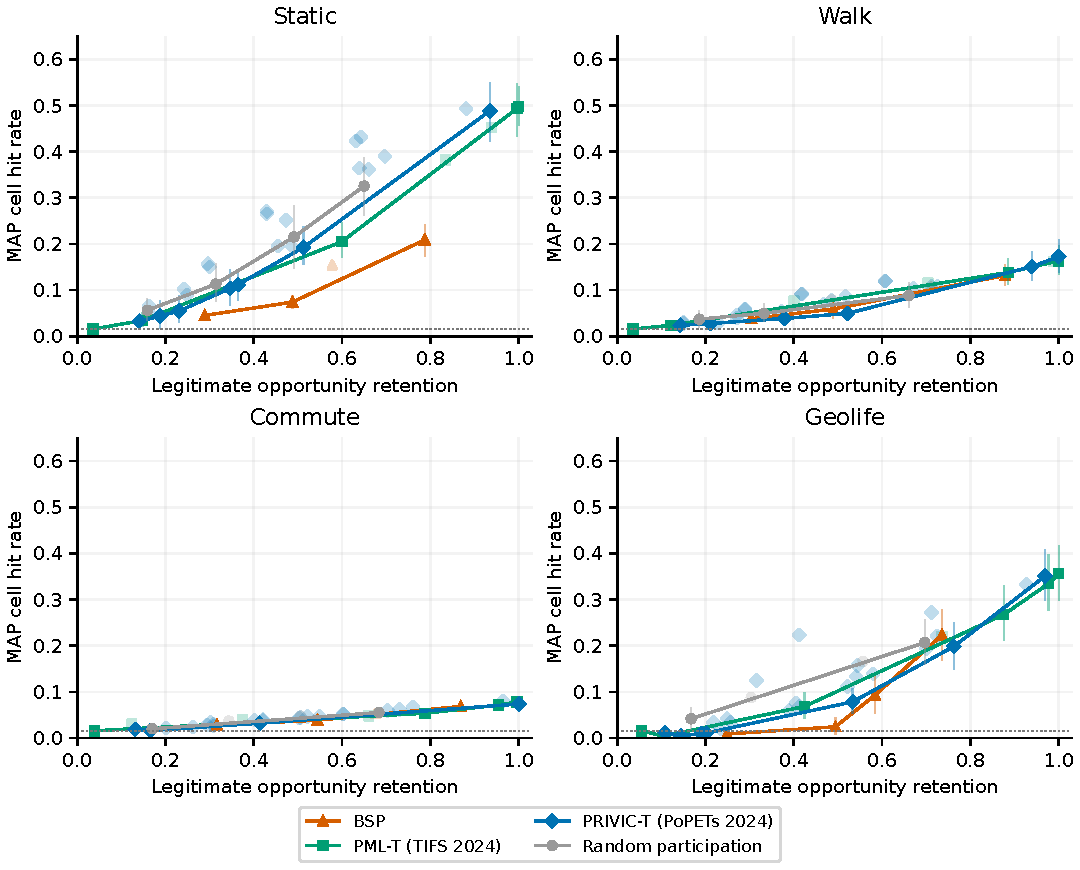
\includegraphics[width=\linewidth]{recent_tradeoff.pdf}
\caption{Recent-method comparison under defense-aware adaptive probes. Faint symbols show all executed settings, including PRIVIC-T thinning; solid lines are each method's lower convex envelope. Error bars at envelope vertices are pointwise 95\% cluster-bootstrap intervals for those executed settings. Envelope-mixture difference intervals are computed separately by paired resampling and envelope reselection, conditional on fixed training. These are exploratory comparisons on the simulated truthful-task interface. Figure~\ref{fig:commute-zoom} repeats the Commute panel on an expanded vertical scale.}
\label{fig:recent}
\end{figure}
\begin{table}[tbp]
\centering\small
\caption{Recent-method envelope comparison at retention 0.5. Values are percentage points; negative differences favor BSP. All rows have 1,000 valid overlapping resamples. These pointwise intervals describe exploratory test-selected envelopes, conditional on the development data and fixed PRIVIC channels; they omit training variability and do not validate deployed policies.}
\label{tab:recent}\begin{tabular}{llrrr}
\toprule
Scenario & Comparator & BSP hit & Other hit & Difference [95\% CI] \\
\midrule
Static & PML-T & 7.96 & 16.74 & -8.77 [-11.38, -6.06] \\
Static & PRIVIC-T & 7.96 & 18.58 & -10.62 [-14.76, -4.70] \\
Walk & PML-T & 6.10 & 8.04 & -1.94 [-3.89, -0.27] \\
Walk & PRIVIC-T & 6.10 & 4.78 & +1.32 [-1.15, +3.29] \\
Commute & PML-T & 3.67 & 3.91 & -0.24 [-0.75, +0.41] \\
Commute & PRIVIC-T & 3.67 & 3.83 & -0.16 [-0.85, +1.01] \\
Geolife & PML-T & 2.89 & 10.19 & -7.30 [-10.23, -3.15] \\
Geolife & PRIVIC-T & 2.89 & 7.16 & -4.28 [-7.52, +0.25] \\
\bottomrule
\end{tabular}
\end{table}

\subsection{Ablation and calibration}
The main runs record no client branch-cap violations for BSP, consistent with its analytical rule and randomized tests. This does not validate the assumed model. The success-only ablation can violate the silence constraint analytically yet attain a smaller empirical hit rate in a finite sample. In replay its hit rate is \GeolifeAblationHit\% at retention \GeolifeAblationRetention\%, versus BSP's \GeolifeBspHit\% at \GeolifeBspRetention\%. The utility levels differ, and the favorable ablation result is retained rather than omitted.

Figure~\ref{fig:calibration} distinguishes posterior concentration from empirical accuracy. BSP's nominal 95\% credible set covers the actual location on only \CommuteBspCoverage\% of periodic-mobility slots; the assumed random walk misses its deterministic structure. Replay coverage is \GeolifeBspCoverage\%. A small maximum in a misspecified posterior is not a distribution-free guarantee about actual location.

\begin{figure}[tbp]
\centering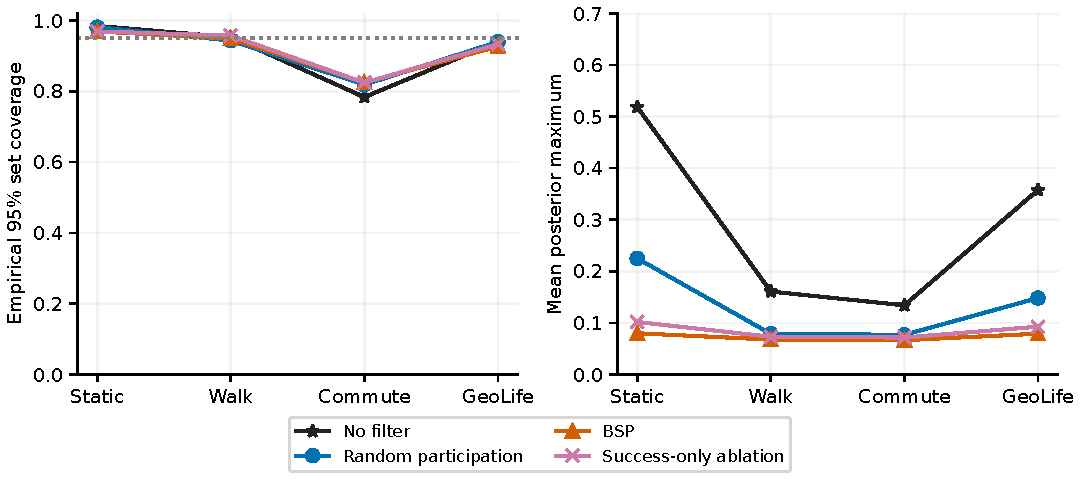
\includegraphics[width=\linewidth]{calibration.pdf}
\caption{Empirical credible-set coverage and mean posterior peak for representative policies. Random participation uses 0.5; BSP and the ablation use threshold 0.1. Scenario means are connected for readability. Nominal credible mass is not promised empirical coverage under mismatch.}
\label{fig:calibration}
\end{figure}

\subsection{Sensitivity and an informed attacker}
Figure~\ref{fig:sensitivity} presents selected sensitivity dimensions; all 72 conditions remain in the artifact. Reduced availability can allow more gate admissions, while movement can spread beliefs and permit later participation. Empirical hit rates need not vary monotonically. BSP retention is 0.109 for grid side 4 and 0.810 for grid side 16, but these are different resolutions and region libraries, not a free privacy improvement at fixed utility semantics. Ideal resets every slot give retention 0.746 and hit rate 0.020; every 12 slots give 0.652 and 0.041. Real identifier rotation may leave linkage clues, which this control assumes away.

\begin{figure}[tbp]
\centering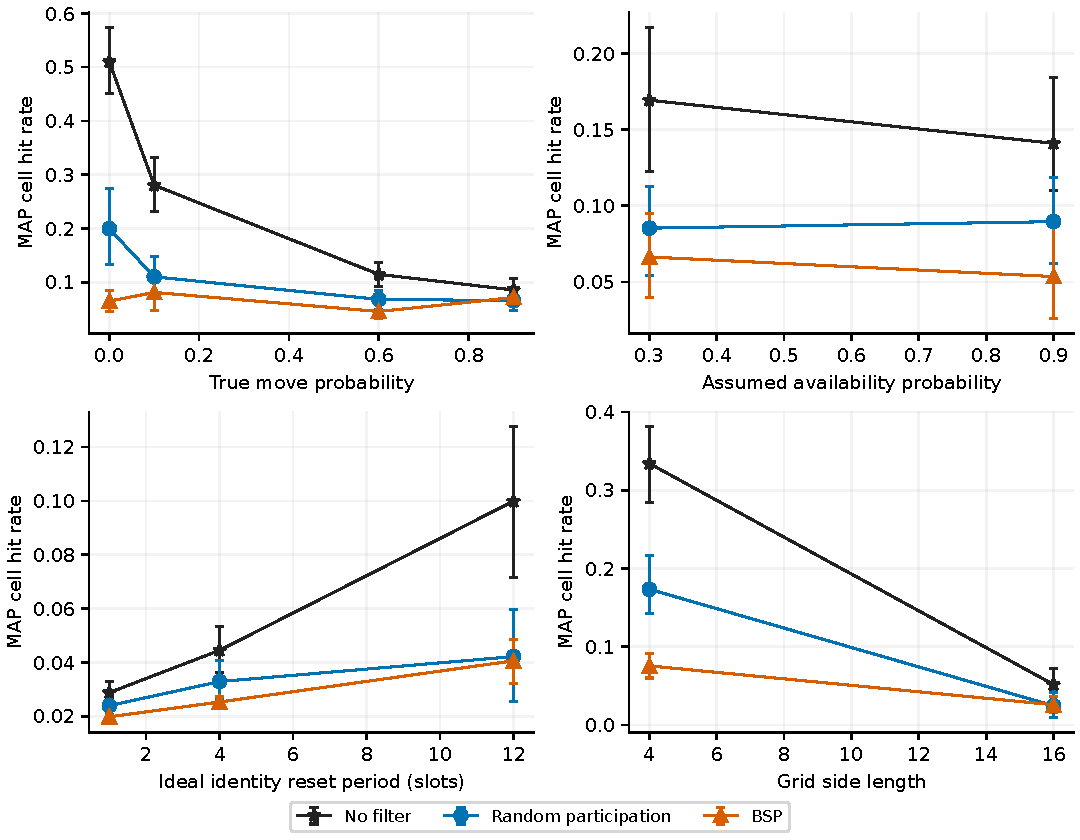
\includegraphics[width=\linewidth]{sensitivity.pdf}
\caption{Selected exploratory sensitivity results. Ten seed clusters contain four users each; error bars are pointwise 95\% bootstrap intervals. Assumed availability is shared by client and attacker in this panel. Identity reset is ideal history erasure. Grid changes alter the target resolution.}
\label{fig:sensitivity}
\end{figure}

Table~\ref{tab:informed} exposes a stronger limitation. With client availability underestimated as 0.3, the informed attacker's peak exceeds 0.1 on 30.0\% of evaluated slots and reaches 0.246, while the client's peak remains capped. When client move probability is overestimated as 0.8, the informed peak exceeds the cap on 41.4\% of slots and reaches 0.263. These findings do not contradict the conditional corollary: shared correct knowledge is absent. They show that a safe-looking client posterior is insufficient against a better-informed observer.

\begin{table}[tbp]
\centering\small
\caption{BSP under better-informed attack. Actual $\alpha=0.648$ and $v=0.3$; one client parameter changes at a time. ``Above cap'' is the descriptive fraction of 1,920 evaluated slots exceeding 0.1, not an independent-sample interval. Client peaks remain within numerical tolerance of 0.1.}
\label{tab:informed}\begin{tabular}{lrrrr}
\toprule
Client mismatch & Retention & MAP hit & Above cap & Largest peak \\
\midrule
$\widehat\alpha=0.3$ & 0.551 & 0.098 & 30.0\% & 0.246 \\
$\widehat\alpha=0.9$ & 0.464 & 0.057 & 8.0\% & 0.164 \\
$\widehat v=0.05$ & 0.457 & 0.038 & 4.7\% & 0.153 \\
$\widehat v=0.8$ & 0.543 & 0.083 & 41.4\% & 0.263 \\
\bottomrule
\end{tabular}
\end{table}

\subsection{Finite-model robustness stress}
Table~\ref{tab:robust} evaluates the new finite-model extension at $\rho=0.1$. Under the nominal client model, both BSP and R-BSP have zero observed attacker local-cap violations. Under all four declared-model mismatches, nominal BSP violates the informed attacker's local cap: 12.6\% of slots when $\alpha$ is underestimated, 2.6\% when it is overestimated, 2.8\% when movement is underestimated, and 14.6\% when movement is overestimated. The corresponding cluster-bootstrap 95\% intervals are $[10.4,15.0]$, $[1.8,3.5]$, $[2.0,3.6]$, and $[13.4,15.8]$ percentage points.

R-BSP records zero local-cap violations in every one of these five conditions because the informed attacker's exact model is included in the nine-member ambiguity set. This is an expected consequence of Proposition~2 and therefore tests implementation and sequential bookkeeping more than it demonstrates generalization beyond the set. The cost is material: R-BSP retains 39.7\% of externally completable normal-task opportunities, compared with 50.9\% for nominal BSP and 46.9--55.2\% for the four misspecified BSP conditions. Its MAP hit rate is 3.47\% versus 4.75--8.49\% for the mismatched nominal policies at this threshold. The robust rule is deliberately conservative; these post-hoc results do not identify an optimal ambiguity set.

\begin{table}[tbp]
\centering\small
\caption{Post-hoc finite-model stress at $\rho=0.1$, 20 synthetic seed clusters and 80 trajectories per row. Viol. is the fraction of 3,840 slot-level outputs per condition for which the informed attacker's posterior exceeds its own local cap. R-BSP contains the attacker's exact $(v,\alpha)=(0.3,0.648)$ model. Retention is Eq.~\eqref{eq:utility}.}
\label{tab:robust}\begin{tabular}{lrrrr}
\toprule
Client model & BSP viol. & R-BSP viol. & BSP retention & R-BSP retention \\
\midrule
Nominal & 0.0\% & 0.0\% & 50.9\% & 39.7\% \\
$\widehat{\alpha}=0.3$ & 12.6\% & 0.0\% & 54.2\% & 39.7\% \\
$\widehat{\alpha}=0.9$ & 2.6\% & 0.0\% & 47.3\% & 39.7\% \\
$\widehat{v}=0.05$ & 2.8\% & 0.0\% & 46.9\% & 39.7\% \\
$\widehat{v}=0.8$ & 14.6\% & 0.0\% & 55.2\% & 39.7\% \\
\bottomrule
\end{tabular}

\end{table}

A separate boundary run shows why the finite-set qualifier is substantive rather than cosmetic. Table~\ref{tab:robust-boundary} uses new seeds and correct attacker models that are not members of $\mathcal M$. For the unlisted interior value $\alpha=0.50$, R-BSP has no observed local-cap violation; for $v=0.50$, two of 3,840 slots violate the local cap (0.052\%, cluster-bootstrap 95\% interval $[0,0.156]$). This empirical interpolation should not be mistaken for a theorem. More importantly, when the correct availability rises outside the ambiguity set to $\alpha=0.98$, R-BSP violates the attacker's local cap on 6.93\% of slots, with interval $[5.70,8.31]$ percentage points. At the outside movement value $v=0.95$, one of 3,840 slots violates (0.026\%, interval $[0,0.078]$). Thus finite-model R-BSP can reduce mismatch sensitivity beyond nominal BSP, but protection is not guaranteed for models outside the declared set.

\begin{table}[tbp]
\centering\small
\caption{Post-hoc boundary characterization at $\rho=0.1$, with 20 new synthetic seed clusters and 80 trajectories per row. ``Interior'' means the correct scalar lies between enumerated ambiguity values but is not itself a member; ``outside'' exceeds the corresponding listed range. Viol. is the informed attacker's local-cap violation rate over 3,840 slots per row.}
\label{tab:robust-boundary}\begin{tabular}{lrrrr}
\toprule
Correct attacker model & BSP viol. & R-BSP viol. & BSP retention & R-BSP retention \\
\midrule
$\alpha=0.50$ (unlisted, interior) & 1.15\% & 0.00\% & 52.6\% & 36.3\% \\
$\alpha=0.98$ (outside set) & 18.33\% & 6.93\% & 50.0\% & 40.4\% \\
$v=0.50$ (unlisted, interior) & 0.65\% & 0.05\% & 54.4\% & 36.4\% \\
$v=0.95$ (outside set) & 0.65\% & 0.03\% & 55.6\% & 35.4\% \\
\bottomrule
\end{tabular}

\end{table}

The stress run also exposes computational cost. On the GitHub-hosted Ubuntu/Python 3.12 validation runner, the mean trajectory-median gate time at $\rho=0.1$ is about 417--423 microseconds for the nine-model R-BSP and 51--52 microseconds for BSP. These timings come from a different machine and software environment than the main-study timing batch, so only the within-run order of magnitude is informative; they are not smartphone measurements or a controlled cross-platform benchmark.

\subsection{Measured computation}
For the 64-cell main grid, the mean of per-trajectory median BSP gate times is approximately 16.8--16.9 microseconds; the mean of per-trajectory 95th percentiles is 18.2--18.7 microseconds. The iterative KL implementation has median summaries of about 326--341 microseconds. These are local Python gate timings, excluding probe search, posterior metrics, loading, and communication. Methods ran in separate batches, so the numbers are descriptive implementation costs, not controlled cross-device speedups. Smartphone latency, energy consumption, and cryptographic execution time were not measured. In the recent extension, condition means of trajectory-median gate times range from 12.1 to 14.0 microseconds for PML-T and 2.0 to 3.0 microseconds for PRIVIC-T. PRIVIC training across all 24 channels takes 182.3 seconds separately; online timings exclude that offline fitting. These batch-specific measurements do not establish a controlled speedup.

\section{Discussion and limitations}
The supported positive finding is narrow: a public-history participation rule can reduce the declared model's inference accuracy while retaining some large-region task opportunities. Checking both possible outputs before participation gives a clear model-conditional bound. Static comparisons provide the clearest recent-baseline evidence. Coarse replay improvements are specific to the uniform-prior inference model and do not bound practical observer accuracy; walk and periodic comparisons show no consistent advantage over both recent comparators.

First, nominal BSP relies on one declared belief model. R-BSP turns this limitation into an explicit finite ambiguity-set guarantee by intersecting member-wise constraints, and the post-hoc stress test shows the expected removal of local-cap violations when the informed attacker's exact model is included. This does not solve model uncertainty in general. The robust-set construction was introduced after nominal failures were known; although the nine parameter combinations reuse levels already present in the earlier stress design, their Cartesian-product use as an ambiguity set was not independently validated. The resulting rule is conservative even when the nominal model is correct and offers no theorem for attackers outside the set. The boundary experiment makes this concrete: an outside-set availability model at $\alpha=0.98$ produces a 6.93\% local-cap violation rate even under R-BSP. A deployment would therefore need a defensible model-set construction procedure---for example from development/validation uncertainty---followed by evaluation that was not used to choose that set.

Second, the model omits informative measurement contents, acknowledgments, payment records, network observations, and within-slot timing. Common-deadline release is a protocol requirement, not an implemented property of a real platform. General collection windows need a state describing visits or acquisition time rather than only the current sampled cell. The on-time probability sweep does not replace such a model.

Third, the data are short, selected, historical, and coarse. One 48-minute window per user does not describe a full day; excluding users without consecutive samples can change the mobility mix. Seventeen test windows have no observed cell change, and small movements within a roughly 4-km cell are invisible. Tasks are simulated on public movement traces. The experiments estimate neither the prevalence of current attacks nor the probability of identifying a home. The development-fitted no-output diagnostic quantifies one weakness of the uniform prior. We have not rerun adaptive probes with that population prior, so neither its incremental leakage nor BSP's resulting utility is established here.

Fourth, the attack is greedy with a fixed probe budget. Longer-horizon task design, coordinated accounts, location-dependent availability, and personalized prior knowledge may change the frontier. The client maximizes current admission rather than future utility. Normal tasks have equal reward; coverage is a simple opportunity-cell proxy rather than measurement reconstruction quality. The region-size breakdown shows that preserved completions primarily serve large regions; fine-region tasks can be excluded entirely. Changes in task scale or reward composition may therefore change the usefulness of the same retention value. Independent account repetitions do not constitute a multi-user allocation or platform-capacity benchmark.

Finally, comparisons depend on finite parameter grids and exploratory interpolation. Bootstrap intervals condition on the selected traces, tasks, and clustering, without resolving distribution shift or multiple testing. The KL and recent-method extensions were added after the main run. Recent policy envelopes are selected on the evaluation set; their bootstrap intervals describe this exploratory selection procedure rather than validating an independently tuned policy. PRIVIC uses one noisy training seed and some IBU/GIBU loops reach their iteration limits; small likelihood gaps do not establish distribution recovery. Its true-eligibility task adapter changes the published output semantics. The full-text comparison with HECTA establishes differences in observations, trust assumptions, and privacy objectives, but does not provide a head-to-head system evaluation or an exhaustive novelty assessment.

\section{Reproducibility and research record}
The local artifact contains configurations, deterministic preprocessing, user splits, hashes, seeds, compressed event logs, trajectory-level rows, analysis code, generated figures, and LaTeX sources. The public-observation module receives no ground truth or future positions. Evaluation logs retain simulator truth for auditing and are not the attack interface. Plots and tabulated numbers are generated from saved results. The post-review prior diagnostic, task-area table, pooled raw completions, and expanded comparison plot are regenerated by \texttt{src.review\_diagnostics}; its input hashes, per-user values, and per-task area records are saved separately from the original simulations.

Twenty-three tests cover posterior branches, nominal and robust gate bounds and maximality, an informed-attacker R-BSP integration case, KL feasibility, transition conservation, unbiased ties, boundaries, duplicates, invalid task deadlines, missing minutes, split separation, paired normal tasks, numerical replay, author-code BA/IBU conformance, PML optimality against a general linear program, vector-valued observation channels, and policy-envelope agreement with a mixture linear program. The corrected pilot, interrupted KL run, and initial shorter PRIVIC training are retained separately and excluded from the final comparisons. Completed runs contain no recorded simulation failures.

The raw GeoLife archive is separately sourced; the study does not claim new collection, anonymization, or unrestricted redistribution. The project repository is available at \url{https://github.com/js110/Bpaper}; it is a version-controlled working repository, not an immutable archival release. Third-party full texts and the raw GeoLife archive are obtained separately from their recorded sources. The supplied author and funding details require author verification; conflicts, contributions, the funders' roles, and any required ethics or data-use determinations remain for responsible authors to supply. AI assistance was used for research organization, code, analysis, drafting, and the two conceptual schematics in Figs.~\ref{fig:architecture} and~\ref{fig:workflow}. Their prompts, original raster files, revision history, and agent visual checks are archived; experimental plots are generated from measured simulation logs. Final disclosure and scientific verification require author review under the selected venue's policy.

\section{Conclusion}
Sequential regional task outputs can reveal location despite local storage of precise coordinates, and probabilistic silence must be included in that analysis. BSP provides a maximal scalar gate for both posterior branches and a sequential cap under explicit model and transition conditions. R-BSP extends that result to a finite public ambiguity set by taking the maximal common scalar gate; when an informed attacker's model is included, the corresponding model-specific branch cap is enforced. The exploratory stress test verifies this behavior but also shows a substantial retention and computation cost, while the boundary run demonstrates that violations can reappear outside the declared ambiguity set. Existing comparisons favor BSP in some settings rather than universally, preserved completions concentrate on large regions, and replay accuracy under a uniform prior is not a practical privacy bound. The contribution is therefore a channel-specific nominal and finite-model robust participation mechanism with reproducible boundary tests, not a guarantee against arbitrary auxiliary knowledge or a complete mobile-crowdsensing privacy system.

\section*{Funding}
This work was supported in part by the Heilongjiang Provincial University Teacher Scientific Research Business Fee under Grant 2018-KYYWF0941, in part by the Heilongjiang Provincial Natural Science Foundation Joint Fund Cultivation Project under Grant PL2024F002, in part by the National Foreign Expert Key Support Project under Grant D2O25O185, and in part by the Heilongjiang Provincial Undergraduate University Excellent Young Teacher Fundamental Research Support Plan under Grant YQJH2024239.

\clearpage
\appendix
\setcounter{figure}{0}
\setcounter{table}{0}
\renewcommand{\theHfigure}{appendix.\arabic{figure}}
\renewcommand{\theHtable}{appendix.\arabic{table}}
\section{Task composition and expanded comparison}
\label{sec:diagnostics}
Table~\ref{tab:task-area} records all normal tasks from the representative BSP settings. Its opportunity counts use simulator eligibility and the shared external-availability draw, whereas completion additionally requires admission. Counts describe the stored finite sample; slots are not independent replicates and no slot-level confidence interval is claimed.
\begin{table}[htbp]
\centering\small
\caption{Post-review task-area breakdown for executed BSP $\rho=0.1$ under adaptive probes. Area is the number of cells in the original 64-cell region library. Retention is completed/opportunities. Counts are pooled over 80 synthetic trajectories or 67 replay users; these are not policy-envelope mixtures.}
\label{tab:task-area}\begin{tabular}{llrrrr}
\toprule
Scenario & Area (cells) & Tasks & Opportunities & Completed & Retention \\
\midrule
Static & 1--8 & 2222 & 55 & 0 & 0.000 \\
Static & 9--31 & 313 & 53 & 22 & 0.415 \\
Static & 32--64 & 344 & 169 & 113 & 0.669 \\
Walk & 1--8 & 2222 & 63 & 0 & 0.000 \\
Walk & 9--31 & 313 & 53 & 13 & 0.245 \\
Walk & 32--64 & 344 & 164 & 124 & 0.756 \\
Commute & 1--8 & 2222 & 57 & 0 & 0.000 \\
Commute & 9--31 & 313 & 45 & 22 & 0.489 \\
Commute & 32--64 & 344 & 157 & 119 & 0.758 \\
Geolife & 1--8 & 1829 & 49 & 0 & 0.000 \\
Geolife & 9--31 & 274 & 59 & 18 & 0.305 \\
Geolife & 32--64 & 281 & 149 & 109 & 0.732 \\
\bottomrule
\end{tabular}

\end{table}

Figure~\ref{fig:commute-zoom} retains every method setting from the Commute panel of Fig.~\ref{fig:recent}, with a different vertical range to make the low-risk portion readable. It does not change the estimates, interval construction, or inconclusive interpretation of the matched-retention differences.
\begin{figure}[htbp]
\centering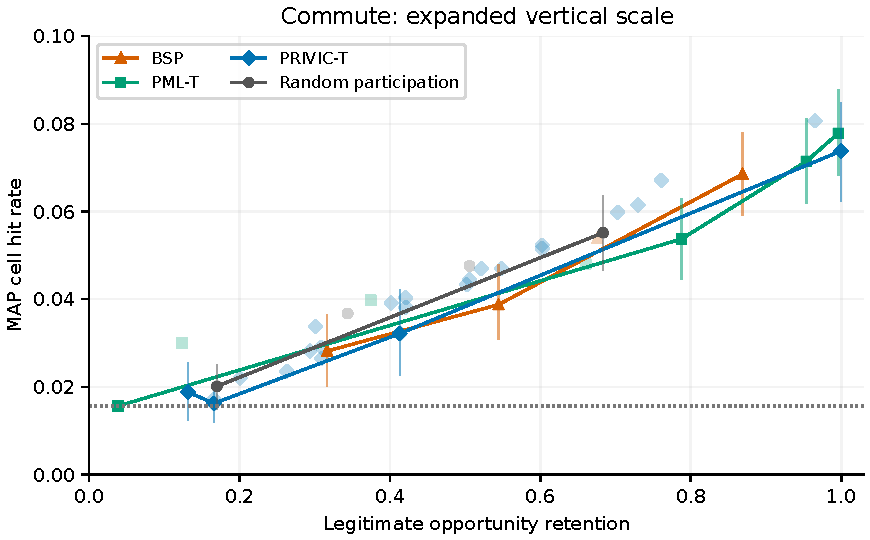
\includegraphics[width=.84\linewidth]{recent_commute_zoom.pdf}
\caption{Expanded Commute comparison (vertical range 0--0.10 rather than 0--0.65). Markers and colors identify methods; faint points are executed settings and lines are test-selected lower envelopes. Vertex error bars are pointwise cluster-bootstrap intervals conditional on fixed training. The dotted line marks uniform-prior expected accuracy.}
\label{fig:commute-zoom}
\end{figure}

\clearpage
\bibliographystyle{elsarticle-num}
\bibliography{references}
\end{document}
